\documentclass[11pt,a4paper]{article}
\usepackage[utf8]{inputenc}
\usepackage[vietnamese]{babel}
\usepackage{amsmath,amssymb}
\usepackage[version=4]{mhchem}
\usepackage{geometry}
\geometry{top=1.5cm,bottom=1.2cm,left=1.4cm,right=1.4cm,headheight=28pt,headsep=12pt,footskip=18pt}
\usepackage{graphicx}
\usepackage{xcolor}
\usepackage{tabularx}
\usepackage{array}
\usepackage{tikz}
\usepackage{fancyhdr}
\usepackage{enumitem}
\usepackage{multido}
\usepackage{tcolorbox}
\usepackage{colortbl}

\definecolor{hfRed}{HTML}{D32F2F}
\definecolor{hfGreen}{HTML}{8BC390}
\definecolor{mainGreen}{HTML}{2E7D32}
\definecolor{solBlue}{HTML}{1565C0}
\definecolor{tableGreen}{HTML}{E8F5E9}

\usepackage{ex_test}

\pagestyle{fancy}
\fancyhf{}
\renewcommand{\headrulewidth}{0.75pt}
\renewcommand{\headrule}{\hbox to\headwidth{\color{hfGreen}\leaders\hrule height \headrulewidth\hfill}}
\renewcommand{\footrulewidth}{0.75pt}
\renewcommand{\footrule}{\hbox to\headwidth{\color{hfGreen}\leaders\hrule height \footrulewidth\hfill}}

\fancyhead[L]{\small\itshape\color{hfRed}Tài liệu lưu hành nội bộ}
\fancyhead[R]{\small\color{hfRed}Thầy \textbf{TRẦN VĂN THẠNH} - 0777.470.803}

\fancyfoot[L]{\footnotesize\itshape\color{hfRed}CS1: 6/15 Nguyễn Hoàng, P. Kim Long, TP Huế \quad|\quad CS2: 24 Đặng Thái Thân, TP Huế}
\fancyfoot[R]{\small\textbf{\color{hfRed}Trang \thepage}}

\setlength{\parindent}{0pt}
\setlength{\parskip}{2pt}

\begin{document}

\begin{minipage}[t]{0.45\textwidth}
\textbf{TỔ LÍ - HÓA}\\
\textbf{ĐỀ CHÍNH THỨC}\\
\textit{(Đề thi có 04 trang)}
\end{minipage}
\hfill
\begin{minipage}[t]{0.52\textwidth}
\raggedleft
\textbf{\color{hfRed}ĐỀ KIỂM TRA GIỮA HỌC KÌ I}\\
\textbf{MÔN: HOÁ HỌC -- LỚP 10}\\
\textit{Thời gian làm bài: 45 phút (không kể thời gian phát đề)}\\
\textbf{MÃ ĐỀ THI: 1201}
\end{minipage}

\vspace{4pt}
\noindent
\textit{Họ và tên thí sinh:} \dotfill \textit{SBD:} \dotfill

\vspace{2pt}
\noindent
\textit{\footnotesize (Cho biết nguyên tử khối: $\ce{H=1; B=10,81; C=12; N=14; O=16; F=19; Ne=20,19; Na=23; Mg=24; P=31; S=32; Cl=35,5; K=39; Ca=40; Fe=56; Br=79,91}$).}

\vspace{2pt}
\begin{center}
\textbf{CHÚ Ý: Học sinh không được sử dụng bảng tuần hoàn các nguyên tố hóa học.}
\end{center}

\vspace{2pt}
\hrule color{hfGreen} height 0.5pt

\vspace{4pt}
\noindent
{\color{mainGreen}\textbf{\Large A. PHẦN TRẮC NGHIỆM (7 ĐIỂM)}}

\vspace{3pt}
\noindent
{\color{mainGreen}\textbf{\large PHẦN I. Câu trắc nghiệm nhiều phương án lựa chọn (3,0 điểm)}}\\
\textit{\small Thí sinh trả lời từ câu 1 đến câu 12. Mỗi câu hỏi thí sinh chỉ chọn một phương án.}
\vspace{2pt}

\begin{ex}
Đường kính của nguyên tử khoảng $10^2\text{ pm}$, trong khi đường kính của hạt nhân khoảng $10^{-2}\text{ pm}$. Đường kính nguyên tử lớn gấp bao nhiêu lần so với đường kính hạt nhân?
\choice
{1000.}
{10000.}
{100.}
{10.}
\end{ex}
\begin{ex}
Số electron tối đa có trong 1 AO p là
\choice
{2.}
{6.}
{3.}
{1.}
\end{ex}
\begin{ex}
Phát biểu nào sau đây không đúng khi nói về vai trò của hóa học đối với đời sống và sản xuất?
\choice
{Nghiên cứu quy luật hình thành, vận động của các thiên thể và địa tầng Trái Đất.}
{Cung cấp phân bón hóa học và thuốc bảo vệ thực vật nhằm tăng năng suất nông nghiệp.}
{Nghiên cứu và sản xuất các loại thuốc chữa bệnh, vắc-xin và vật tư y tế.}
{Tạo ra các sản phẩm tiêu dùng thiết yếu như xà phòng, chất tẩy rửa và chất dẻo.}
\end{ex}
\begin{ex}
X là nguyên tố s. Trong bảng tuần hoàn, X có thể thuộc nhóm
\choice
{IB.}
{VIA.}
{IA.}
{VIB.}
\end{ex}
\begin{ex}
Trong bảng tuần hoàn các nguyên tố hóa học do nhà hóa học người Nga D. I. Mendeleev (1834 -- 1907) đề xuất năm 1869, các nguyên tố được sắp xếp theo chiều tăng dần của
\choice
{số hiệu nguyên tử.}
{số electron hóa trị.}
{bán kính nguyên tử.}
{khối lượng nguyên tử.}
\end{ex}
\begin{ex}
Bảng tuần hoàn các nguyên tố hóa học hiện nay gồm có
\choice
{6 chu kì và 16 nhóm.}
{8 chu kì và 18 nhóm.}
{7 chu kì và 18 cột.}
{7 chu kì và 8 nhóm.}
\end{ex}
\begin{ex}
Hạt mang điện trong hạt nhân nguyên tử là
\choice
{neutron và electron.}
{electron.}
{proton.}
{neutron.}
\end{ex}
\begin{ex}
Cho các phát biểu về sự chuyển động của electron trong nguyên tử như sau:\\
(a) Theo mô hình hành tinh nguyên tử, các electron chuyển động xung quanh hạt nhân theo những quỹ đạo tròn hay bầu dục.\\
(b) Theo mô hình hiện đại, các electron chuyển động rất nhanh xung quanh hạt nhân theo một quỹ đạo xác định tạo thành đám mây electron.\\
(c) Theo mô hình hiện đại, trong nguyên tử, electron chuyển động rất nhanh, không theo quỹ đạo xác định.\\
(d) Theo mô hình hiện đại, xác suất tìm thấy electron tại mỗi điểm trong không gian của AO là 90\%.\\
Số phát biểu đúng là
\choice
{1.}
{4.}
{2.}
{3.}
\end{ex}
\begin{ex}
Trong nguyên tử, vùng không gian bao quanh hạt nhân và mang điện tích âm được tạo nên bởi các hạt
\choice
{proton.}
{electron.}
{neutron.}
{alpha.}
\end{ex}
\begin{ex}
Kí hiệu phân lớp electron nào sau đây không đúng?
\choice
{3p.}
{3s.}
{3f.}
{3d.}
\end{ex}
\begin{ex}
Phát biểu nào sau đây không đúng?
\choice
{Khối lượng hạt electron nhỏ hơn nhiều so với khối lượng hạt proton.}
{Khối lượng nguyên tử tập trung chủ yếu ở lớp vỏ.}
{Trong nguyên tử, khối lượng tập trung chủ yếu ở hạt nhân.}
{Hạt proton và hạt neutron có khối lượng gần bằng nhau.}
\end{ex}
\begin{ex}
Cho các nguyên tử: $^{12}_6\ce{X}, ^{14}_7\ce{Y}, ^{14}_6\ce{Z}, ^{24}_{12}\ce{T}$. Các nguyên tử thuộc cùng một nguyên tố hóa học là
\choice
{\ce{X} và \ce{Z}.}
{\ce{X} và \ce{T}.}
{\ce{Y} và \ce{Z}.}
{\ce{Z} và \ce{T}.}
\end{ex}
\vspace{4pt}
\noindent
{\color{mainGreen}\textbf{\large PHẦN II. Câu trắc nghiệm đúng sai (2,0 điểm)}}\\
\textit{\small Thí sinh trả lời từ câu 1 đến câu 2. Trong mỗi ý a), b), c), d) ở mỗi câu, thí sinh chọn đúng hoặc sai.}
\vspace{2pt}

\begin{ex}
Fluorine và hợp chất của nó được sử dụng làm chất chống sâu răng, chất cách điện, chất làm lạnh, vật liệu chống dính, \dots\ Nguyên tử fluorine (\ce{F}) chứa 9 electron và có số khối là 19.
\choiceTF
{Hạt nhân nguyên tử \ce{F} có 9 proton và 10 neutron}
{Nguyên tử \ce{F} có điện tích lớp vỏ là +9}
{Khối lượng của một nguyên tử \ce{F} xấp xỉ 28 amu}
{Phân tử $\ce{RF2}$ có tổng số hạt mang điện là 60. Nguyên tử của nguyên tố R có 2 electron thuộc lớp M và R là nguyên tố kim loại}
\end{ex}
\begin{ex}
Boron (\ce{B}) là nguyên tố có nhiều tác dụng đối với cơ thể người như: làm lành vết thương, điều hoà nội tiết sinh dục, chống viêm khớp, \dots\ Do ngọn lửa cháy có màu đặc biệt nên boron vô định hình được dùng làm pháo hoa. Boron có hai đồng vị là $^{10}_5\ce{B}$ và $^{11}_5\ce{B}$, nguyên tử khối trung bình là 10,81.
\choiceTF
{Hai đồng vị của boron có cùng số proton nhưng khác nhau về số neutron}
{Nguyên tố \ce{B} thuộc chu kì 3 trong bảng tuần hoàn}
{Nguyên tử của nguyên tố \ce{B} có 4 electron s và có 3 electron ở phân lớp ngoài cùng}
{Phần trăm số nguyên tử của đồng vị $^{10}_5\ce{B}$ trong tự nhiên là 81\%}
\end{ex}
\vspace{4pt}
\noindent
{\color{mainGreen}\textbf{\large PHẦN III. Câu trắc nghiệm yêu cầu trả lời ngắn (2,0 điểm)}}\\
\textit{\small Thí sinh trả lời từ câu 1 đến câu 4.}
\vspace{2pt}

\begin{ex}
Cho biết tổng số hạt proton, neutron và electron trong một nguyên tử của nguyên tố $^{39}_{19}\ce{K}$ là bao nhiêu?
\par\textbf{Trả lời:} \dotfill\end{ex}
\begin{ex}
Nguyên tử của nguyên tố calcium ($Z = 20$) có bao nhiêu lớp electron?
\par\textbf{Trả lời:} \dotfill\end{ex}
\begin{ex}
Cho các nguyên tử sau: $\ce{X}\ (Z = 11); \ce{Y}\ (Z = 17); \ce{Z}\ (Z = 20); \ce{T}\ (Z = 26)$. Có bao nhiêu nguyên tố thuộc loại nguyên tố s?
\par\textbf{Trả lời:} \dotfill\end{ex}
\begin{ex}
Trong tự nhiên, nguyên tố bromine có 2 đồng vị là $^{79}_{35}\ce{Br}$ và $^{81}_{35}\ce{Br}$. Nguyên tử khối trung bình của bromine là 79,91. Trong hợp chất $\ce{NaBrO}_x$, nguyên tử đồng vị $^{81}\ce{Br}$ chiếm 30,994\% về khối lượng. Giá trị của $x$ là bao nhiêu (với O và Na là các đồng vị $^{16}_8\ce{O}, ^{23}_{11}\ce{Na}$)?
\par\textbf{Trả lời:} \dotfill\end{ex}
\vspace{6pt}
\noindent
{\color{mainGreen}\textbf{\Large B. PHẦN TỰ LUẬN (3 ĐIỂM)}}
\vspace{3pt}

\begin{ex}
\textbf{(1,0 điểm)} Phosphorus (P) là một nguyên tố dinh dưỡng khoáng thiết yếu cho sự phát triển của cây trồng, thường có mặt trong các loại phân bón NPK. Trong bảng tuần hoàn, nguyên tố phosphorus có số hiệu nguyên tử là 15.\\
a) Viết cấu hình electron nguyên tử của P ở trạng thái cơ bản.\\
b) Xác định vị trí của P (chu kì và nhóm) trong bảng tuần hoàn, cho biết P thuộc loại nguyên tố nào (s, p hay d)?

\vspace{0.3cm}
\dotfill\\
\dotfill\\
\dotfill\\
\dotfill
\end{ex}
\begin{ex}
\textbf{(1,0 điểm)} Neon (Ne) là một nguyên tố khí hiếm, phát ra ánh sáng đỏ cam đặc trưng khi có phóng điện qua khí ở áp suất thấp và được ứng dụng trong một số loại biển hiệu phát sáng. Neon có ba đồng vị bền và tỉ lệ phần trăm số nguyên tử các đồng vị của Ne được xác định theo phổ khối lượng như hình sau:
\begin{center}
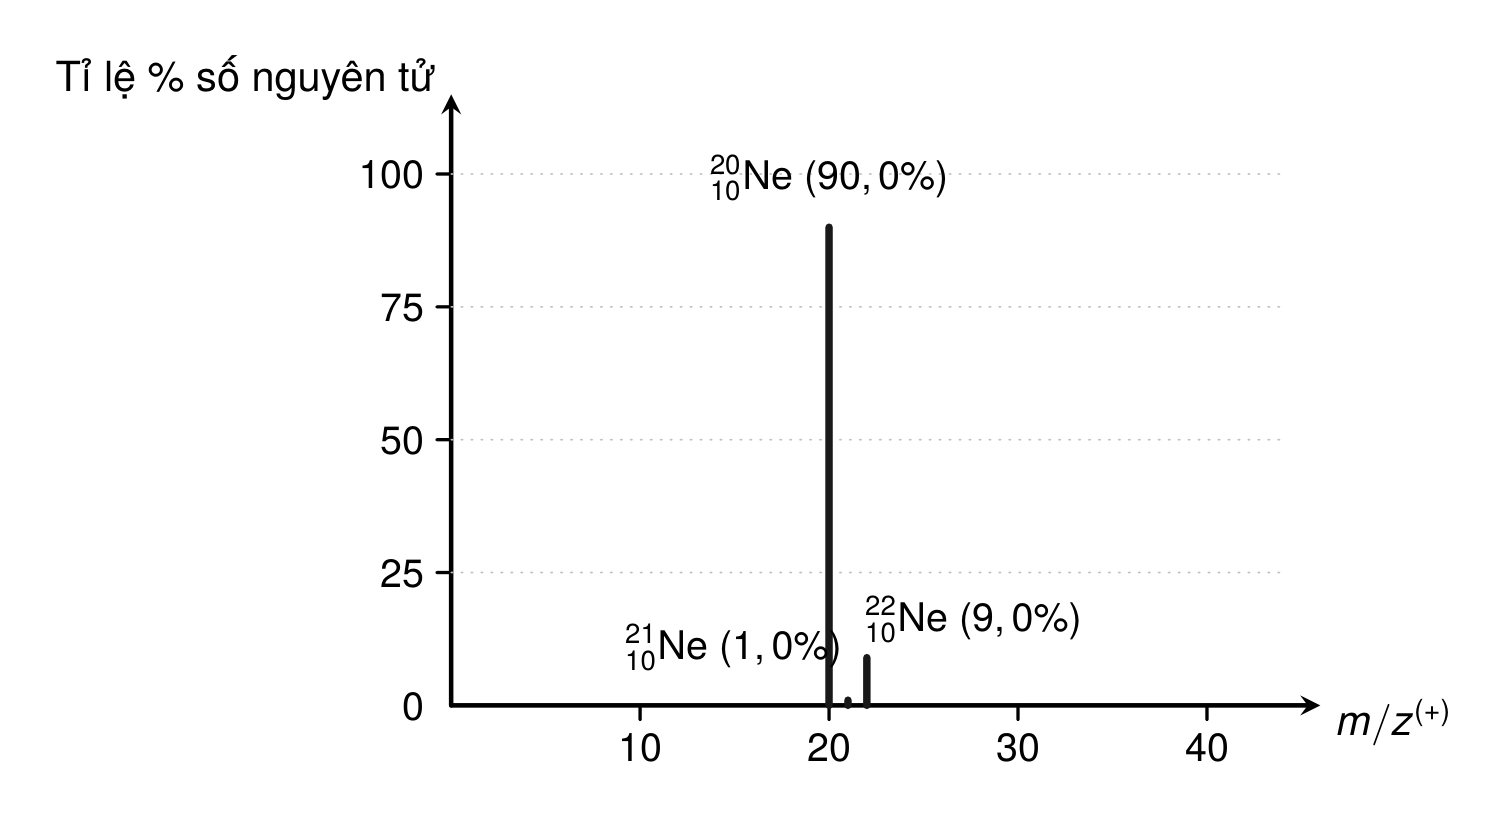
\includegraphics[width=8.5cm]{images_hoa10/pho_khoi_luong_neon_1201.png}
\end{center}
a) Tính nguyên tử khối trung bình của Neon (kết quả làm tròn đến hàng phần trăm).\\
b) Tính số nguyên tử của mỗi loại đồng vị còn lại khi có 1 nguyên tử $^{21}_{10}\ce{Ne}$ (kết quả làm tròn đến hàng đơn vị).\\
c) Tính thể tích của 10 gam Ne ở điều kiện chuẩn ($25^\circ\text{C}$, 1 bar) (kết quả làm tròn đến hàng phần mười).

\vspace{0.3cm}
\dotfill\\
\dotfill\\
\dotfill\\
\dotfill\\
\dotfill
\end{ex}
\begin{ex}
\textbf{(1,0 điểm)} Nguyên tố R thuộc nhóm A trong bảng tuần hoàn. Nguyên tử R có tổng số electron ở các phân lớp s là 7 và tổng số electron ở lớp ngoài cùng là 1.\\
a) Viết cấu hình electron đầy đủ của nguyên tử R. Dự đoán tính chất hóa học cơ bản của nguyên tố R (kim loại hay phi kim) và giải thích.\\
b) Phân tử $\ce{R2XY4}$ có tổng số hạt proton là 86. Biết nguyên tố X và Y thuộc cùng một nhóm A và ở hai chu kì liên tiếp trong bảng tuần hoàn. Hãy xác định số hiệu nguyên tử của X và Y.

\vspace{0.3cm}
\dotfill\\
\dotfill\\
\dotfill\\
\dotfill\\
\dotfill
\end{ex}
\vspace{6pt}
\begin{center}
\textbf{---------- HẾT ----------}\\
\textit{\small - Thí sinh không được sử dụng tài liệu.\\
- Cán bộ coi thi không giải thích gì thêm.}
\end{center}
\end{document}
